


\tikzset{every picture/.style={line width=0.75pt}} %set default line width to 0.75pt        

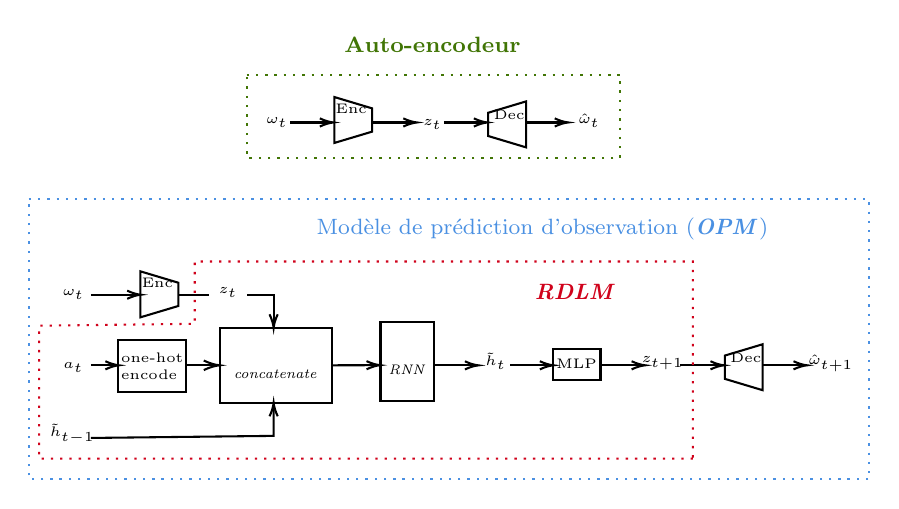
\begin{tikzpicture}[x=0.75pt,y=0.75pt,yscale=-1,xscale=1]
    %uncomment if require: \path (0,2102); %set diagram left start at 0, and has height of 2102

    %Straight Lines [id:da7945271061326031] 
    \draw    (100,1800) -- (111.5,1800) ;
    \draw [shift={(113.5,1800)}, rotate = 180] [color={rgb, 255:red, 0; green, 0; blue, 0 }  ][line width=0.75]    (6.56,-1.97) .. controls (4.17,-0.84) and (1.99,-0.18) .. (0,0) .. controls (1.99,0.18) and (4.17,0.84) .. (6.56,1.97)   ;
    %Straight Lines [id:da710289636295716] 
    \draw    (100,1835) -- (188,1834) -- (188,1820) ;
    \draw [shift={(188,1818)}, rotate = 90] [color={rgb, 255:red, 0; green, 0; blue, 0 }  ][line width=0.75]    (6.56,-1.97) .. controls (4.17,-0.84) and (1.99,-0.18) .. (0,0) .. controls (1.99,0.18) and (4.17,0.84) .. (6.56,1.97)   ;
    %Straight Lines [id:da9775676154282154] 
    \draw    (146.38,1800) -- (160,1800) ;
    \draw [shift={(162,1800)}, rotate = 180] [color={rgb, 255:red, 0; green, 0; blue, 0 }  ][line width=0.75]    (7.65,-2.3) .. controls (4.86,-0.97) and (2.31,-0.21) .. (0,0) .. controls (2.31,0.21) and (4.86,0.98) .. (7.65,2.3)   ;
    %Straight Lines [id:da789934339782699] 
    \draw    (100,1766) -- (122,1766) ;
    \draw [shift={(124,1766)}, rotate = 180] [color={rgb, 255:red, 0; green, 0; blue, 0 }  ][line width=0.75]    (6.56,-1.97) .. controls (4.17,-0.84) and (1.99,-0.18) .. (0,0) .. controls (1.99,0.18) and (4.17,0.84) .. (6.56,1.97)   ;
    %Shape: Trapezoid [id:dp2317709974845179] 
    \draw   (123.84,1754.74) -- (142.07,1760.21) -- (142.07,1771.42) -- (123.84,1776.88) -- cycle ;
    %Straight Lines [id:da7383754609221514] 
    \draw    (142,1766) -- (188,1766) -- (188,1780) ;
    \draw [shift={(188,1782)}, rotate = 270] [color={rgb, 255:red, 0; green, 0; blue, 0 }  ][line width=0.75]    (6.56,-1.97) .. controls (4.17,-0.84) and (1.99,-0.18) .. (0,0) .. controls (1.99,0.18) and (4.17,0.84) .. (6.56,1.97)   ;
    %Straight Lines [id:da49394763541143527] 
    \draw    (216,1800) -- (237.33,1799.94) ;
    \draw [shift={(239.33,1799.94)}, rotate = 179.85] [color={rgb, 255:red, 0; green, 0; blue, 0 }  ][line width=0.75]    (6.56,-1.97) .. controls (4.17,-0.84) and (1.99,-0.18) .. (0,0) .. controls (1.99,0.18) and (4.17,0.84) .. (6.56,1.97)   ;
    %Straight Lines [id:da8738633046359771] 
    \draw    (265.89,1800.03) -- (284.72,1800.03) ;
    \draw [shift={(286.72,1800.03)}, rotate = 180] [color={rgb, 255:red, 0; green, 0; blue, 0 }  ][line width=0.75]    (6.56,-1.97) .. controls (4.17,-0.84) and (1.99,-0.18) .. (0,0) .. controls (1.99,0.18) and (4.17,0.84) .. (6.56,1.97)   ;
    %Straight Lines [id:da3021616845453272] 
    \draw    (302,1800) -- (320.83,1800) ;
    \draw [shift={(322.83,1800)}, rotate = 180] [color={rgb, 255:red, 0; green, 0; blue, 0 }  ][line width=0.75]    (6.56,-1.97) .. controls (4.17,-0.84) and (1.99,-0.18) .. (0,0) .. controls (1.99,0.18) and (4.17,0.84) .. (6.56,1.97)   ;
    %Straight Lines [id:da8984410115217915] 
    \draw    (346,1800) -- (353.4,1800) -- (365.04,1800) ;
    \draw [shift={(367.04,1800)}, rotate = 180] [color={rgb, 255:red, 0; green, 0; blue, 0 }  ][line width=0.75]    (6.56,-1.97) .. controls (4.17,-0.84) and (1.99,-0.18) .. (0,0) .. controls (1.99,0.18) and (4.17,0.84) .. (6.56,1.97)   ;
    %Shape: Trapezoid [id:dp37639710819638017] 
    \draw   (423.61,1812) -- (405.38,1806.53) -- (405.38,1795.32) -- (423.61,1789.86) -- cycle ;
    %Straight Lines [id:da10289425963982124] 
    \draw    (384,1800) -- (403.04,1800) ;
    \draw [shift={(405.04,1800)}, rotate = 180] [color={rgb, 255:red, 0; green, 0; blue, 0 }  ][line width=0.75]    (6.56,-1.97) .. controls (4.17,-0.84) and (1.99,-0.18) .. (0,0) .. controls (1.99,0.18) and (4.17,0.84) .. (6.56,1.97)   ;
    %Straight Lines [id:da12692360321469986] 
    \draw    (424,1800) -- (443.04,1800) ;
    \draw [shift={(445.04,1800)}, rotate = 180] [color={rgb, 255:red, 0; green, 0; blue, 0 }  ][line width=0.75]    (6.56,-1.97) .. controls (4.17,-0.84) and (1.99,-0.18) .. (0,0) .. controls (1.99,0.18) and (4.17,0.84) .. (6.56,1.97)   ;
    %Shape: Trapezoid [id:dp27180057752038367] 
    \draw   (217.23,1670.74) -- (235.46,1676.21) -- (235.46,1687.42) -- (217.23,1692.88) -- cycle ;
    %Shape: Trapezoid [id:dp9437628483591106] 
    \draw   (309.61,1695) -- (291.38,1689.53) -- (291.38,1678.32) -- (309.61,1672.86) -- cycle ;
    %Straight Lines [id:da19635385567867214] 
    \draw    (310,1683) -- (328,1683) ;
    \draw [shift={(330,1683)}, rotate = 180] [color={rgb, 255:red, 0; green, 0; blue, 0 }  ][line width=0.75]    (6.56,-1.97) .. controls (4.17,-0.84) and (1.99,-0.18) .. (0,0) .. controls (1.99,0.18) and (4.17,0.84) .. (6.56,1.97)   ;
    %Straight Lines [id:da6136759960935583] 
    \draw    (196,1683) -- (214.83,1683) ;
    \draw [shift={(216.83,1683)}, rotate = 180] [color={rgb, 255:red, 0; green, 0; blue, 0 }  ][line width=0.75]    (6.56,-1.97) .. controls (4.17,-0.84) and (1.99,-0.18) .. (0,0) .. controls (1.99,0.18) and (4.17,0.84) .. (6.56,1.97)   ;
    %Straight Lines [id:da5198115307428596] 
    \draw    (236,1683) -- (255.04,1683) ;
    \draw [shift={(257.04,1683)}, rotate = 180] [color={rgb, 255:red, 0; green, 0; blue, 0 }  ][line width=0.75]    (6.56,-1.97) .. controls (4.17,-0.84) and (1.99,-0.18) .. (0,0) .. controls (1.99,0.18) and (4.17,0.84) .. (6.56,1.97)   ;
    %Straight Lines [id:da6362560665768464] 
    \draw    (270,1683) -- (289.04,1683) ;
    \draw [shift={(291.04,1683)}, rotate = 180] [color={rgb, 255:red, 0; green, 0; blue, 0 }  ][line width=0.75]    (6.56,-1.97) .. controls (4.17,-0.84) and (1.99,-0.18) .. (0,0) .. controls (1.99,0.18) and (4.17,0.84) .. (6.56,1.97)   ;
    %Shape: Rectangle [id:dp3864765488610862] 
    \draw  [color={rgb, 255:red, 74; green, 144; blue, 226 }  ,draw opacity=1 ][dash pattern={on 0.84pt off 2.51pt}] (70,1720) -- (475,1720) -- (475,1855) -- (70,1855) -- cycle ;
    %Shape: Rectangle [id:dp17767261593347572] 
    \draw  [color={rgb, 255:red, 65; green, 117; blue, 5 }  ,draw opacity=1 ][dash pattern={on 0.84pt off 2.51pt}] (175,1660) -- (355,1660) -- (355,1700) -- (175,1700) -- cycle ;
    %Shape: Polygon [id:ds8294746409292746] 
    \draw  [color={rgb, 255:red, 208; green, 2; blue, 27 }  ,draw opacity=1 ][dash pattern={on 0.84pt off 2.51pt}] (390,1845) -- (75,1845) -- (75,1780.92) -- (150,1780) -- (150,1750) -- (390,1750) -- cycle ;


    % Text Node
    \draw (333.5,1764.5) node  [color={rgb, 255:red, 208; green, 2; blue, 27 }  ,opacity=1 ] [align=left] {\footnotesize \textbf{\textit{RDLM}}};
    % Text Node
    \draw (317.5,1734.5) node  [color={rgb, 255:red, 74; green, 144; blue, 226 }  ,opacity=1 ] [align=left] {\footnotesize Modèle de prédiction d'observation (\textbf{\textit{OPM}})};
    % Text Node
    \draw (264.5,1645.5) node  [color={rgb, 255:red, 65; green, 117; blue, 5 }  ,opacity=1 ] [align=left] {{\footnotesize \textbf{Auto-encodeur}}};
    % Text Node
    \draw (189.5,1683) node  [font=\tiny] [align=left] {$\displaystyle \omega _{t}$};
    % Text Node
    \draw (340,1682) node  [font=\tiny] [align=left] {$\displaystyle \hat{\omega }_{t}$};
    % Text Node
    \draw (301.5,1679.5) node   [align=left] {{\tiny Dec}};
    % Text Node
    \draw (225.38,1676.5) node   [align=left] {{\tiny Enc}};
    % Text Node
    \draw (264.5,1684) node  [font=\tiny] [align=left] {$\displaystyle z_{t}$};
    % Text Node
    \draw (456.54,1799) node  [font=\tiny] [align=left] {$\displaystyle \hat{\omega }_{t+1}$};
    % Text Node
    \draw (415.5,1796.5) node   [align=left] {{\tiny Dec}};
    % Text Node
    \draw (375.5,1799) node  [font=\tiny] [align=left] {$\displaystyle z_{t+1}$};
    % Text Node
    \draw (132,1760.5) node   [align=left] {{\tiny Enc}};
    % Text Node
    \draw (295,1798) node  [font=\tiny] [align=left] {$\displaystyle \tilde{h}_{t}$};
    % Text Node
    \draw    (239.48,1779) -- (265.48,1779) -- (265.48,1817) -- (239.48,1817) -- cycle  ;
    \draw (252.48,1798) node  [font=\tiny] [align=left] {\begin{minipage}[lt]{14.99pt}\setlength\topsep{0pt}
            \begin{center}
                \phantom{X}\\\textit{RNN}
            \end{center}

        \end{minipage}};
    % Text Node
    \draw  [color={rgb, 255:red, 255; green, 255; blue, 255 }  ,draw opacity=1 ][fill={rgb, 255:red, 255; green, 255; blue, 255 }  ,fill opacity=1 ]  (157.5,1757) -- (174.5,1757) -- (174.5,1773) -- (157.5,1773) -- cycle  ;
    \draw (166,1765) node  [font=\tiny] [align=left] {$\displaystyle z_{t}$};
    % Text Node
    \draw    (162,1782) -- (216,1782) -- (216,1818) -- (162,1818) -- cycle  ;
    \draw (189,1800) node  [font=\tiny] [align=left] {\begin{minipage}[lt]{34pt}\setlength\topsep{0pt}
            \begin{center}
                \phantom{X}\\\textit{concatenate}
            \end{center}

        \end{minipage}};
    % Text Node
    \draw (91,1833) node  [font=\tiny] [align=left] {$\displaystyle \tilde{h}_{t-1}$};
    % Text Node
    \draw (91.5,1801) node  [font=\tiny] [align=left] {$\displaystyle a_{t}$};
    % Text Node
    \draw (91.5,1766) node  [font=\tiny] [align=left] {$\displaystyle \omega _{t}$};
    % Text Node
    \draw    (322.5,1792) -- (345.5,1792) -- (345.5,1807) -- (322.5,1807) -- cycle  ;
    \draw (334,1799.5) node  [font=\tiny] [align=left] {MLP};
    % Text Node
    \draw    (113,1788) -- (146,1788) -- (146,1813) -- (113,1813) -- cycle  ;
    \draw (129.5,1800.5) node  [font=\tiny] [align=left] {one-hot\\encode};


\end{tikzpicture}